%!TEX program = xelatex 
\documentclass[hyperref, UTF8
,bookmarksnumbered=true, oneside]{ctexbook}
\hypersetup{
            bookmarksnumbered=true,
            bookmarksopen=true,
            colorlinks=false, 
            pdfborder=001,   
				%menucolor=green,%uunknown
				linktocpage=true,%make the link of the content on the number of page
            linkcolor=green,
            anchorcolor=green,
            citecolor=green}
\usepackage{geometry}
\usepackage{tocbibind}
\usepackage{graphicx}
\usepackage{amsmath}
\usepackage{amsfonts}
\usepackage{amssymb}
\usepackage{bm}
\CTEXsetup[name={(,)}]{chapter}
%\CTEXsetup[number={\chinese{section}}]{section}


\newcommand{\beqt}{\begin{equation}}
\newcommand{\eeqt}{\end{equation}}
\newcommand{\beqtnt}{\begin{equation*}}
\newcommand{\eeqtnt}{\end{equation*}}

\geometry{a4paper,centering,scale=0.8}

\title{\huge{软件工程课程作业}\\ \Huge \textbf{Mathematica Input Assistant} \\\phantom{aaa} \\\Huge{用户手册}}
\author{\\ \phantom{aaa} \\\phantom{aaa} \\ \phantom{aaa}\\\\\\\huge{待定小组}\\\\ \Large{基科物理32{  }蒋文韬}\\ \Large{基科物理32{ }张思源{ }}\\ \Large{基科应用31{ }李泽清{ }} \\ \Large{基科应用31 { }傅笛{ }} }
\begin{document}\Large

\frontmatter
\maketitle 

\tableofcontents

\mainmatter

\chapter{引言}

	\section{编写目的} % (fold)

		Mathematica是一款类似MatLab的科学计算软件,与MatLab相比扩展功能与包较少,但符号计算功能十分强大,并且绘图效果更佳,学习数学与物理方向的同学较为常用。然而,Mathematica界面十分简单,与office软件等不同,其众多功能不是展示在用户眼前的,用户需要对能够完成他们需求的函数与代码比较熟悉。对没用过的人与初学者来说与记事本看起来一样,让人无从下手。对偶尔用一用mathematica的人,常常忘记以前用过的函数的具体名称,或者需调节的一些参数的名称与取值。另外,在Mathematica自带帮助里查找想用的函数较为不便,查找函数的参数更是十分繁多,并且帮助为英文,不便英文能力较差的使用者使用。

		因此,我们想做的是一个通过GUI实现的Mathematica输入助手,可将Mathematica的函数作为一个树结构归类显示,并对每个函数类与类中的函数都有简介与示例代码供用户拷贝进Mathematica软件运行。点选某个函数后,便可看见函数的一些常见参数与参数的简单描述,并可在下拉选项框中选择可能的参数值。选择函数并设置好参数后,即可点击生成对应的Mathematica代码,可直接拷贝进入Mathematica运行。
		
	% section 编写目的 (end)

	\section{前景} % (fold)

		Mathematica 是美国 Wolfram Research 公司开发的优秀数学软件,它是当今世
界用于科技计算的难得的一个完全集成环境下的符号运算系统.它拥有的不仅是
数值计算能力,还有强大的符号推导能力, 但由于界面过于简洁,不便于刚刚接触
科研的学生或者有相关计算需求的初学者使用,本产品通过输入助手的方式,
为 Mathematica 的使用者提供一个更加便捷的输入输出工具,方便初学者使用,
在越来越多的大学生学习使用 Mathematica 进行计算的现实背景下,本产品有不
错的发展潜力和需求。
		
	% section 前景 (end)


	

	% section 源代码地址 (end)


\chapter{软件综述}

	\section{软件功能} % (fold)
	本软件的主要功能有:
	\label{sec:}
		\begin{itemize}
			\item 用户通过树形结构与函数简介能够找到想用的函数
			\item 用户可通过函数参数的简介设置参数,生成可直接拷贝进 Mathematica 中使
用的代码
			\item 用户可自行添加自己的函数类与函数
			\item 函数类与函数的信息通过文件保存与读取
			\item 用户可通过函数名搜索函数并点击使用
		\end{itemize}
	% section  (end)
	
	\section{运行环境} % (fold)
		

		本产品可在 Windows 7, Windows 8,Windows 10 系统下运行

\chapter{界面及操作说明}

	\section{主界面} % (fold)

		\begin{figure}[!h]
			\centering
			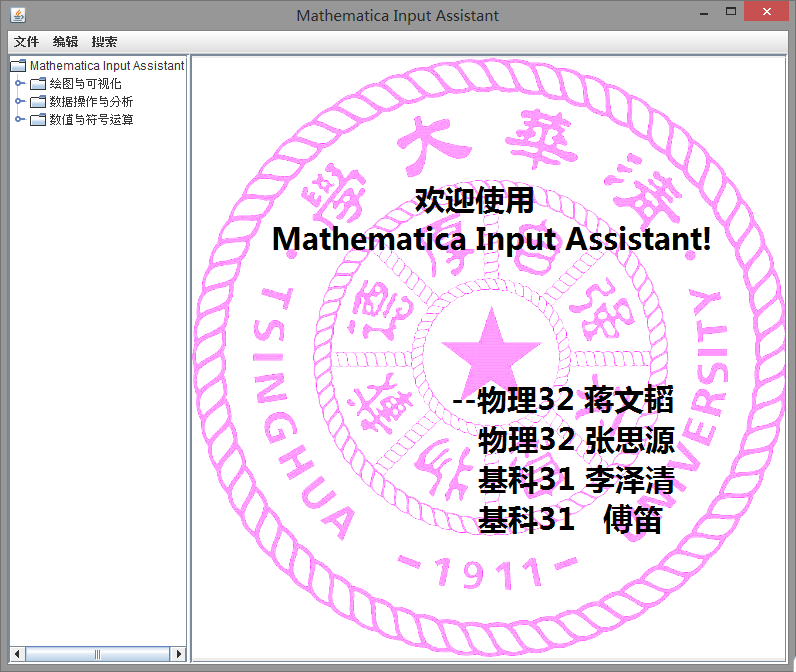
\includegraphics[width=5in]{Welcome.png}
			\caption{主界面效果图}	
		\end{figure}

		主界面如图所示,主要由菜单栏,左侧界面与右侧界面组成。左侧界面为包含所有函数类与函数的树形结构,供用户查找包含其想使用的功能的函数类与函数。右侧界面在未选中任何函数类或函数时为默认的欢迎界面。
		
	% section 主界面 (end)
	\section{菜单栏} % (fold)

		\begin{figure}[!h]
			\begin{minipage}[b]{0.3\textwidth}
			\centering
			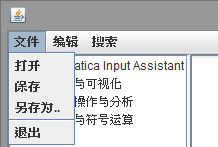
\includegraphics[width=1.7in]{Menu1.png}
			\label{pic:MathPack}
			\end{minipage}%
			\hspace{0.025\textwidth}%
			\begin{minipage}[b]{0.3\textwidth}
			\centering
			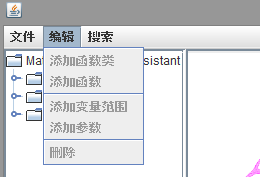
\includegraphics[width=1.7in]{Menu2.png}
			\label{pic:GUIPack}
			\end{minipage}			
			\hspace{0.025\textwidth}%
			\begin{minipage}[b]{0.3\textwidth}
			\centering
			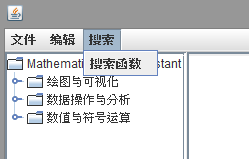
\includegraphics[width=1.7in]{Menu3.png}
			\label{pic:GUIPack}
			\end{minipage}
			\caption{菜单栏效果图}
		\end{figure}

		菜单栏主要由三个子栏组成,如图所示。在未选中任何函数类或函数的情况下时,编辑栏中的选项均为不可用。选中函数类或函数时,启用的选项会相应变化。

	% section 菜单栏 (end)


	\section{左侧界面} % (fold)

		\begin{figure}[!h]
			\begin{minipage}[b]{0.15\textwidth}
			\centering
			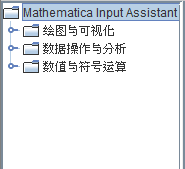
\includegraphics[width=1in]{Left1.png}
			\label{pic:MathPack}
			\end{minipage}%
			\hspace{0.025\textwidth}%
			\begin{minipage}[b]{0.15\textwidth}
			\centering
			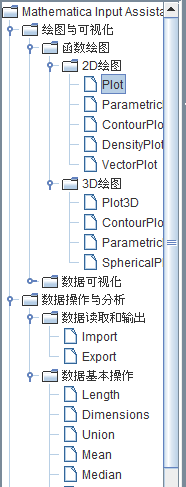
\includegraphics[width=1in]{Left2.png}
			\label{pic:GUIPack}
			\end{minipage}			
			\hspace{0.025\textwidth}%
			\begin{minipage}[b]{0.6\textwidth}
			\centering
			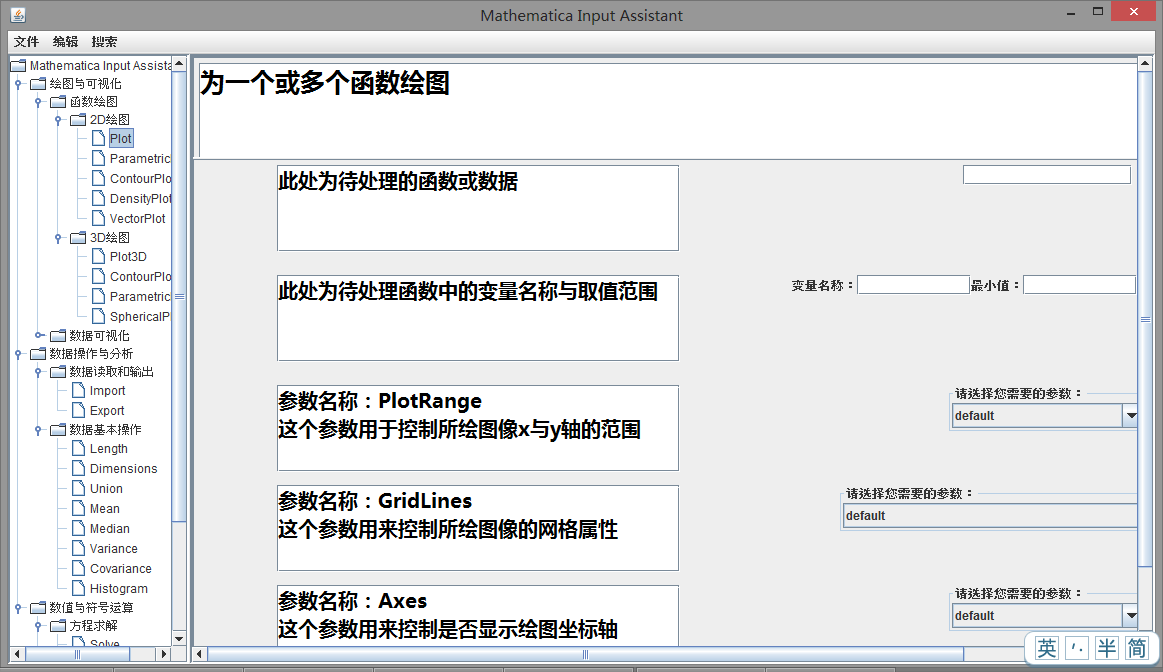
\includegraphics[width=4in]{Left3.png}
			\label{pic:GUIPack}
			\end{minipage}
			\caption{左侧界面效果图}
		\end{figure}

		左侧界面为包含所有函数类与函数的树形结构,供用户查找包含其想使用的功能的函数类与函数。当展开节点较多时,会出现滚动条使用户可以拖动以查看完整的树形结构。当点击相应节点时,右侧界面能够有相应的响应。
		
	% section 左侧界面 (end)

	\section{介绍界面} % (fold)

		\begin{figure}[!h]
			\begin{minipage}[b]{0.45\textwidth}
			\centering
			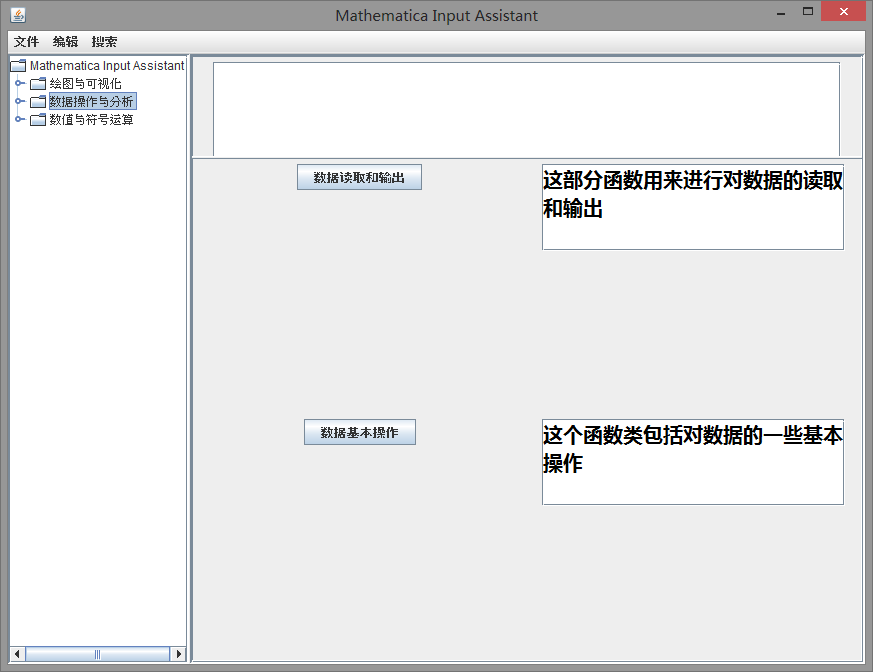
\includegraphics[width=3in]{Right01.png}
			\label{pic:MathPack}
			\end{minipage}%
			\hspace{0.1\textwidth}%
			\begin{minipage}[b]{0.45\textwidth}
			\centering
			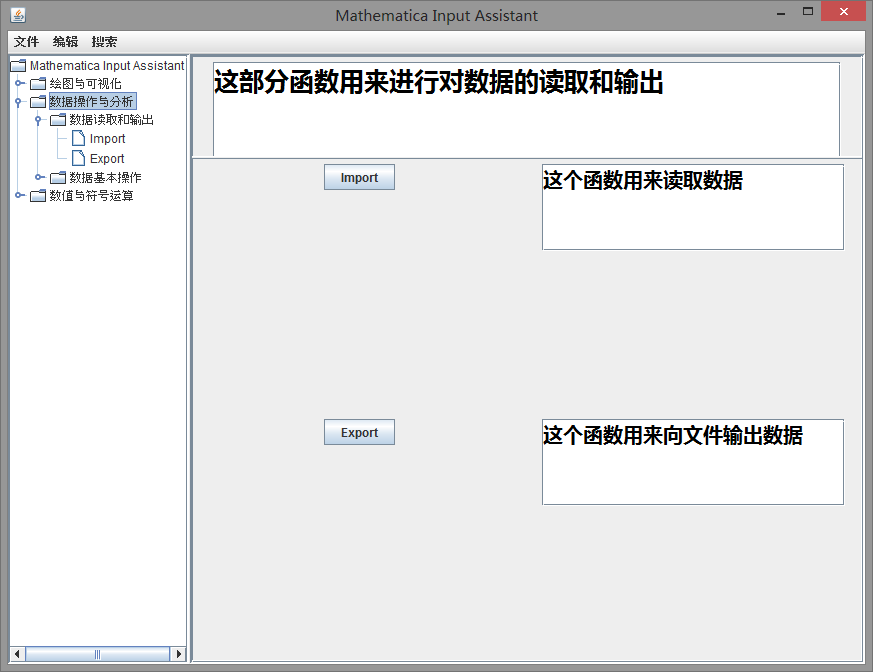
\includegraphics[width=3in]{Right02.png}
			\label{pic:GUIPack}
			\end{minipage}
			\caption{介绍界面效果图}
		\end{figure}

		介绍界面为显示被选中的函数类下的函数类与函数的名称与简介。其中名称对应的按钮可以点击并发生相应跳转。同时,左侧节点的展开情况也会发生相应变化。


		
	% section 介绍界面 (end)

	\section{函数设定界面} % (fold)


		\begin{figure}[!h]
			\begin{minipage}[b]{0.45\textwidth}
			\centering
			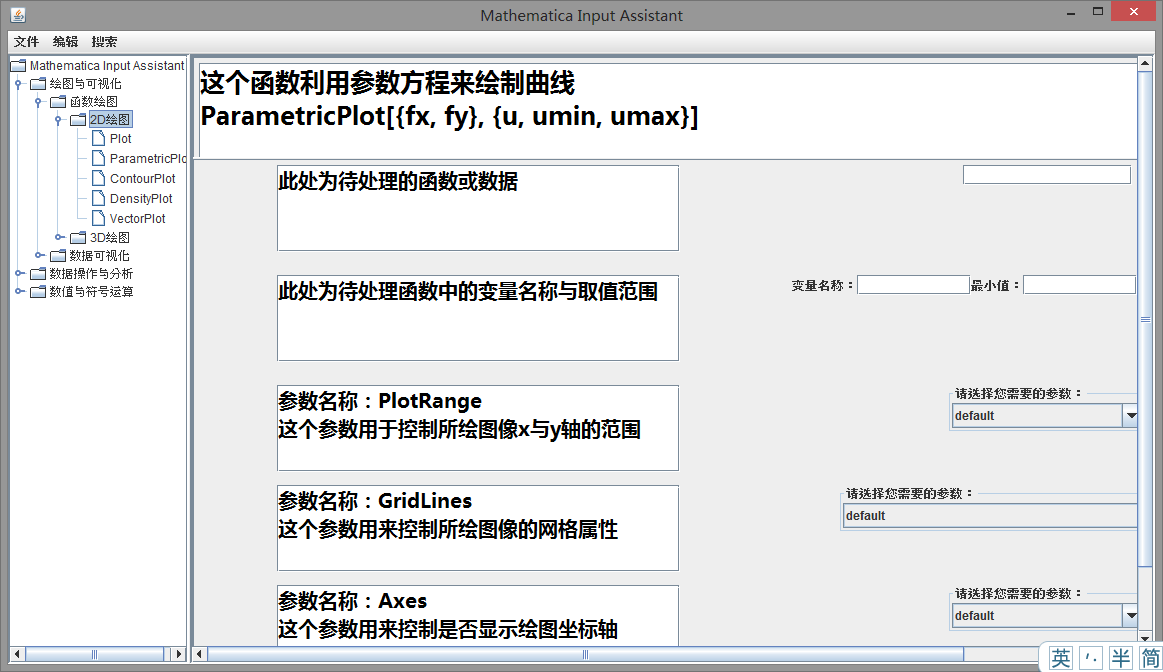
\includegraphics[width=3in]{Right2.png}
			\label{pic:MathPack}
			\end{minipage}%
			\hspace{0.1\textwidth}%
			\begin{minipage}[b]{0.45\textwidth}
			\centering
			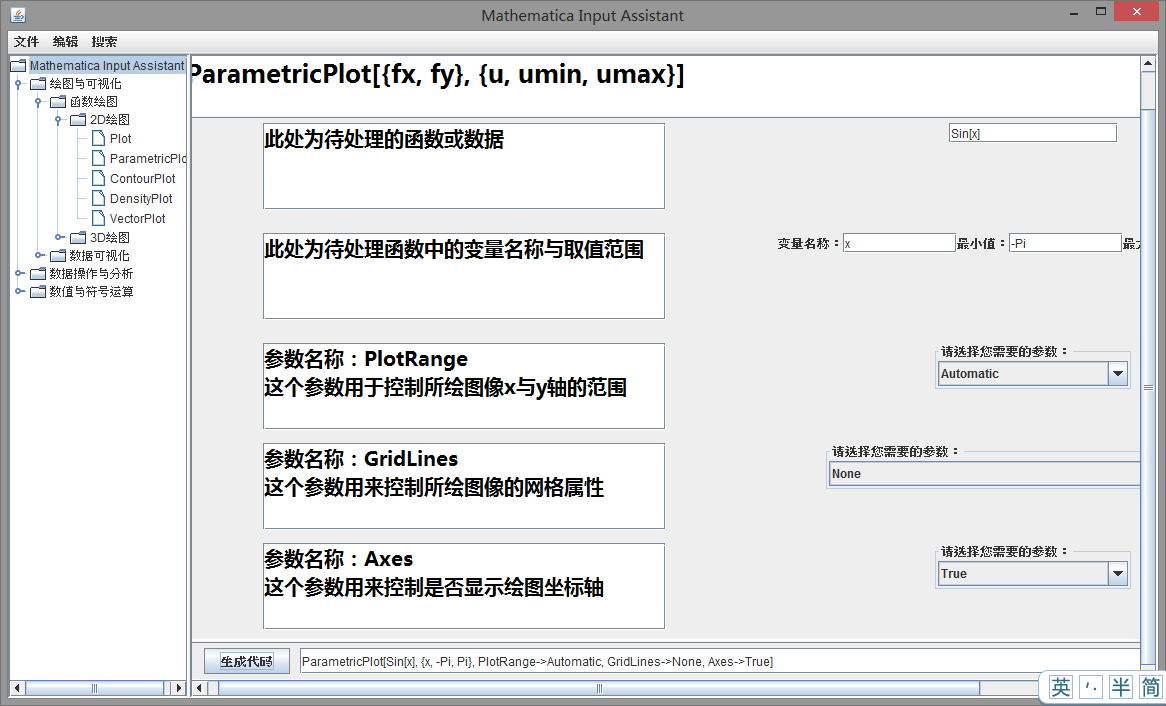
\includegraphics[width=3in]{Right3.png}
			\label{pic:GUIPack}
			\end{minipage}
			\caption{函数设定界面效果图}
		\end{figure}

		函数设定界面可显示出该函数所需的所有参数以及相应说明,供用户设定。当用户设定了所需的参数后,即可通过点击生成代码,生成出可直接拷贝到Mathematica中直接运行的代码,如上图所示。

		
	% section 函数设定界面 (end)

	\section{弹出界面与对话框} % (fold)
		
		\subsection{添加函数类,函数与参数界面} % (fold)

			\begin{figure}[!h]
				\begin{minipage}[b]{0.3\textwidth}
				\centering
				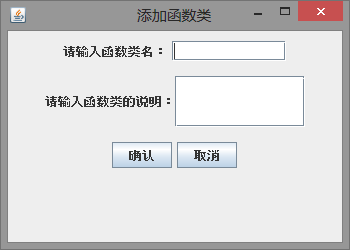
\includegraphics[width=1.7in]{AddFuncClass.png}
				\label{pic:MathPack}
				\end{minipage}%
				\hspace{0.025\textwidth}%
				\begin{minipage}[b]{0.3\textwidth}
				\centering
				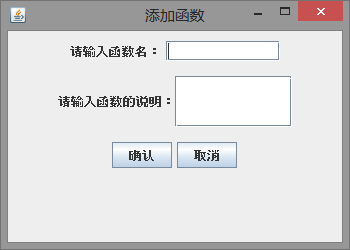
\includegraphics[width=1.7in]{AddMathFunc.png}
				\label{pic:GUIPack}
				\end{minipage}			
				\hspace{0.025\textwidth}%
				\begin{minipage}[b]{0.3\textwidth}
				\centering
				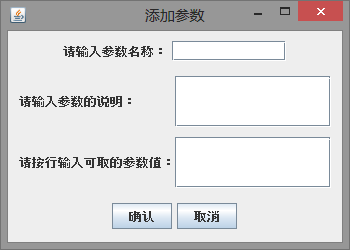
\includegraphics[width=1.7in]{AddPara.png}
				\label{pic:GUIPack}
				\end{minipage}
				\caption{添加功能弹窗效果图}
			\end{figure}

			当用户选择添加函数类、函数和参数时,会弹出如上对话框。用户按照对话框上的说明进行输入即可,而且并
且对于函数名会检查用户输入是否合理,否则会弹窗提醒。成功添加后
即可在右下界面看到变化。

		% subsection 添加函数类界面 (end)

		\subsection{添加变量对话框,删除对话框与搜索对话框} % (fold)

			\begin{figure}[!h]
				\begin{minipage}[b]{0.3\textwidth}
				\centering
				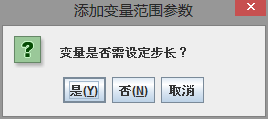
\includegraphics[width=1.7in]{AddVR.png}
				\label{pic:MathPack}
				\end{minipage}%
				\hspace{0.025\textwidth}%
				\begin{minipage}[b]{0.3\textwidth}
				\centering
				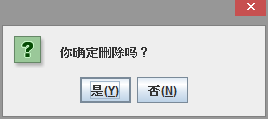
\includegraphics[width=1.7in]{Delete.png}
				\label{pic:GUIPack}
				\end{minipage}			
				\hspace{0.025\textwidth}%
				\begin{minipage}[b]{0.3\textwidth}
				\centering
				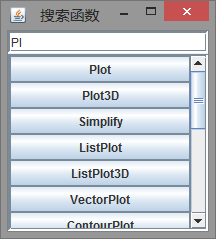
\includegraphics[width=1.7in]{Search.png}
				\label{pic:GUIPack}
				\end{minipage}
				\caption{添加变量,删除与搜索对话框效果图}
			\end{figure}

			添加变量,删除与搜索对话框如图所示。其中搜索对话框的搜索结果会随用户输入而实时变化,搜索结果较多时会出现滚动条。点击某一个搜索结果,搜索框即会消失,并且主面板的右侧将跳转至选中的搜索结果所对应的函数的设置界面。
			
		% subsection 添加变量对话框 (end)

	% section 弹出界面 (end)
	
\chapter{操作说明}
	\section{使用函数}
		假设我们要使用$ParametricPlot$,用户可以在右侧上面部分按照提示进行输入和选择,可以进入如下界面:
		\begin{figure}[!h]
                	\centering
                	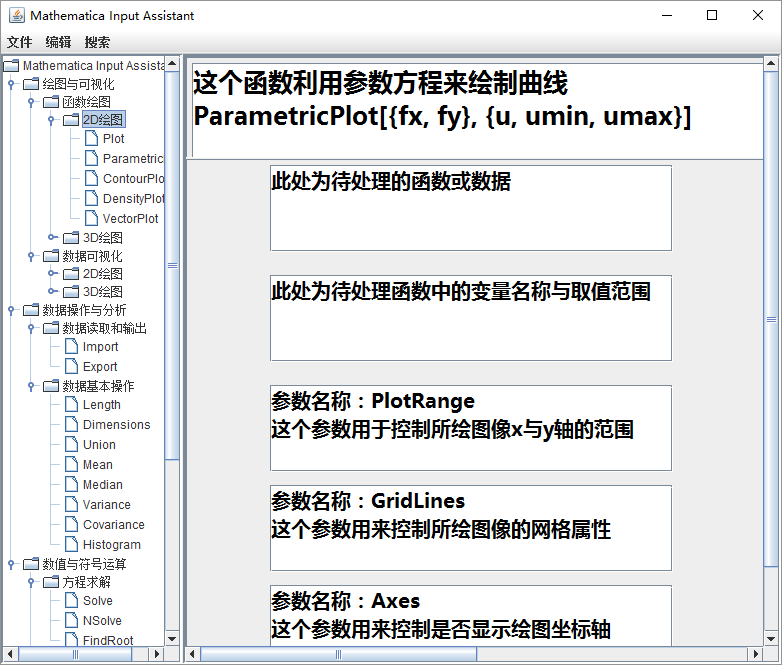
\includegraphics[width=5in]{5.png}
                	\caption{函数使用界面}    
                	\label{pic:MathObject}
            	\end{figure}
		

		点击生成代码然后拷入Mathematica中运行,显示所要画图功能。效果如下:
		\bigskip
		\bigskip
		\begin{figure}[!h]
	        \begin{minipage}[b]{0.45\textwidth}
            \centering
            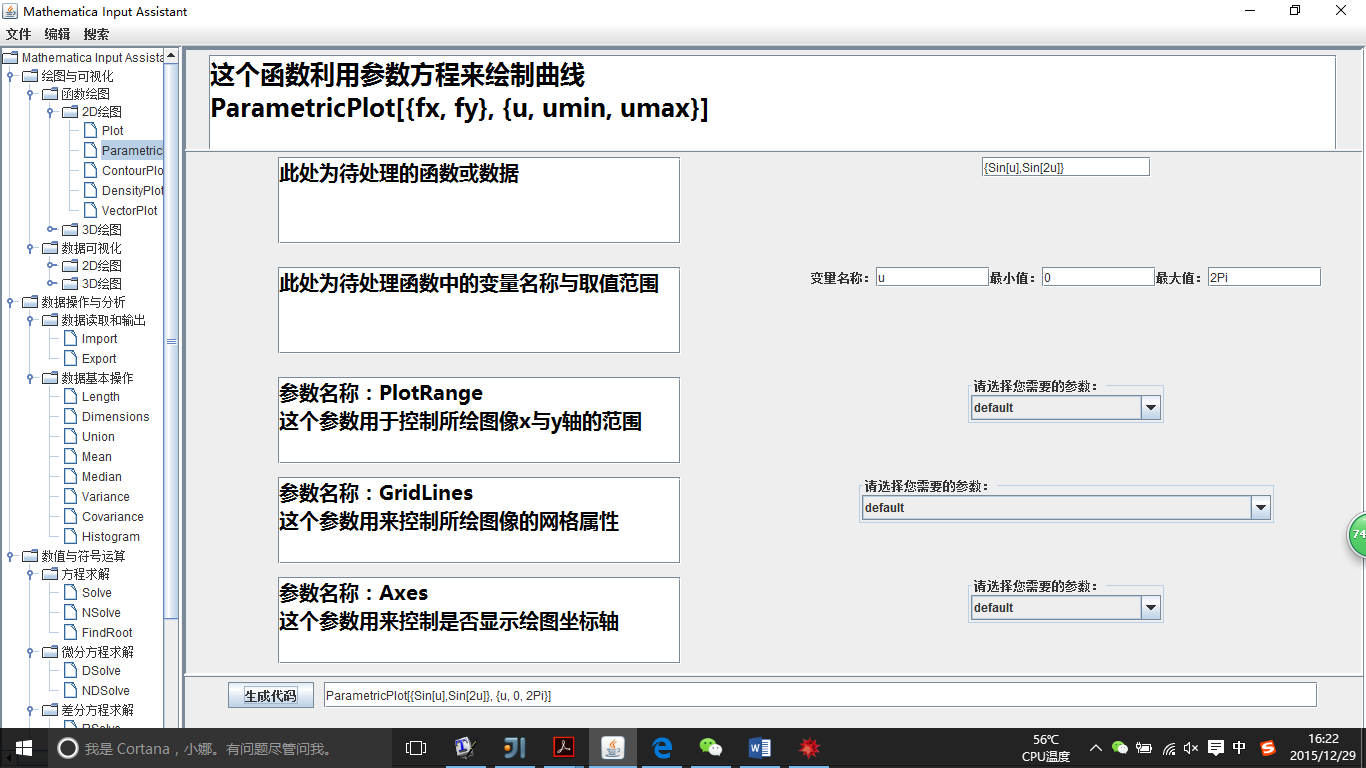
\includegraphics[width=3in]{6.png}
	        \caption{按提示进行输入和选择生成代码}
	        \label{pic:MathPack}
	        \end{minipage}%
	        \hspace{0.1\textwidth}%
	        \begin{minipage}[b]{0.45\textwidth}
	        \centering
	        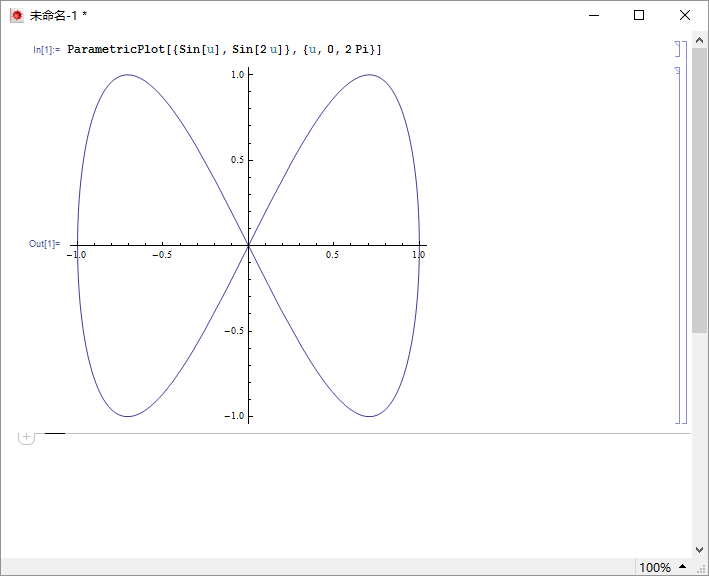
\includegraphics[width=3in]{7.png}
	        \caption{拷入Mathematica中运行}
	        \label{pic:GUIPack}
	        \end{minipage}
        \end{figure}
        \bigskip
        \bigskip
    \section{添加函数与函数类}
    首先在菜单栏选择添加函数进一步添加参数和自变量取值
	范围,如图输入,在右侧上面部分按照提示进行输入和选择,点击生
	成代码然后拷入Mathematica中运行,显示所要画图功能。

	\bigskip
	\bigskip
	\bigskip
	\begin{figure}[!h]
	                \begin{minipage}[b]{0.45\textwidth}
	                \centering
	                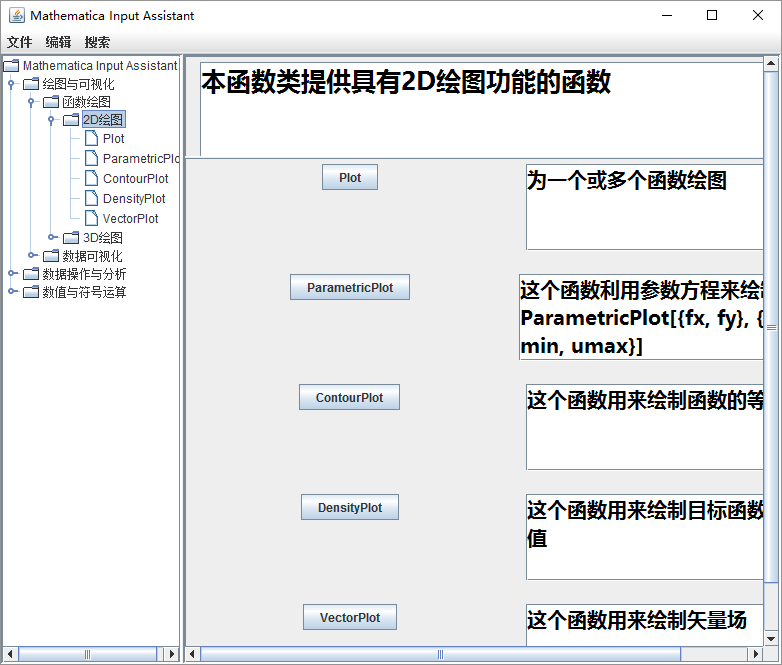
\includegraphics[width=3in]{10.png}
	                \caption{选择添加函数所在函数类}
	                \label{pic:MathPack}
	                \end{minipage}%
	                \hspace{0.1\textwidth}%
	                \begin{minipage}[b]{0.45\textwidth}
	                \centering
	                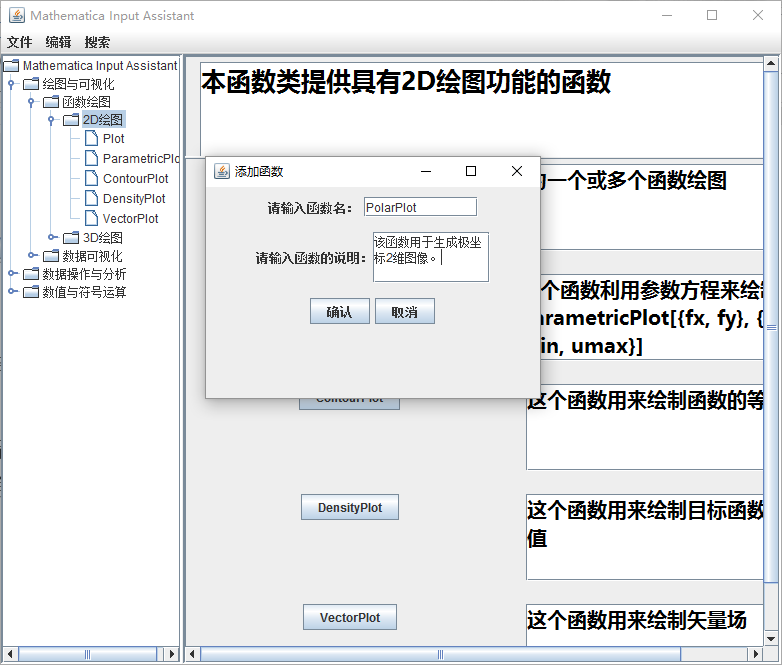
\includegraphics[width=3in]{11.png}
	                \caption{选择添加函数}
	                \label{pic:GUIPack}
	                \end{minipage}
            	\end{figure}

            	\begin{figure}[!h]
	                \begin{minipage}[b]{0.45\textwidth}
	                \centering
	                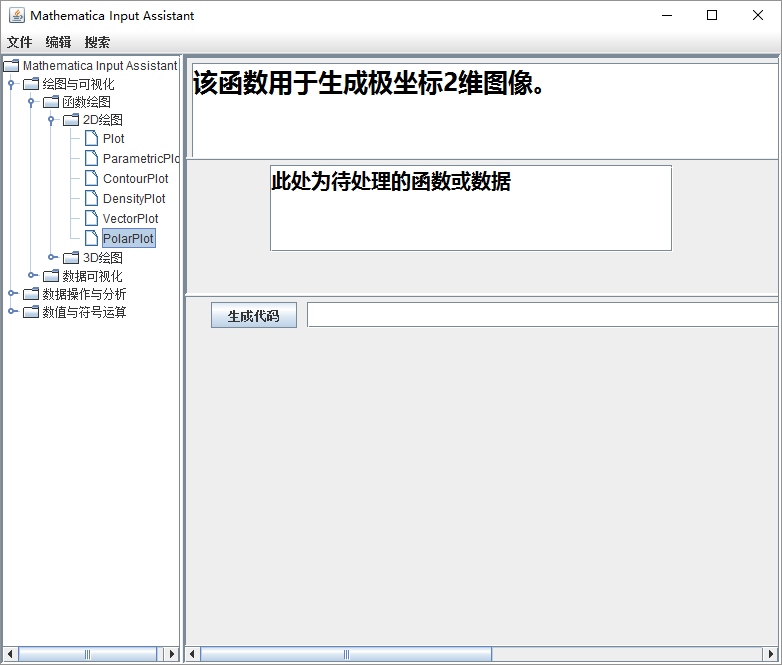
\includegraphics[width=3in]{12.png}
	                \caption{显示所添加函数}
	                \label{pic:MathPack}
	                \end{minipage}%
	                \hspace{0.1\textwidth}%
	                \begin{minipage}[b]{0.45\textwidth}
	                \centering
	                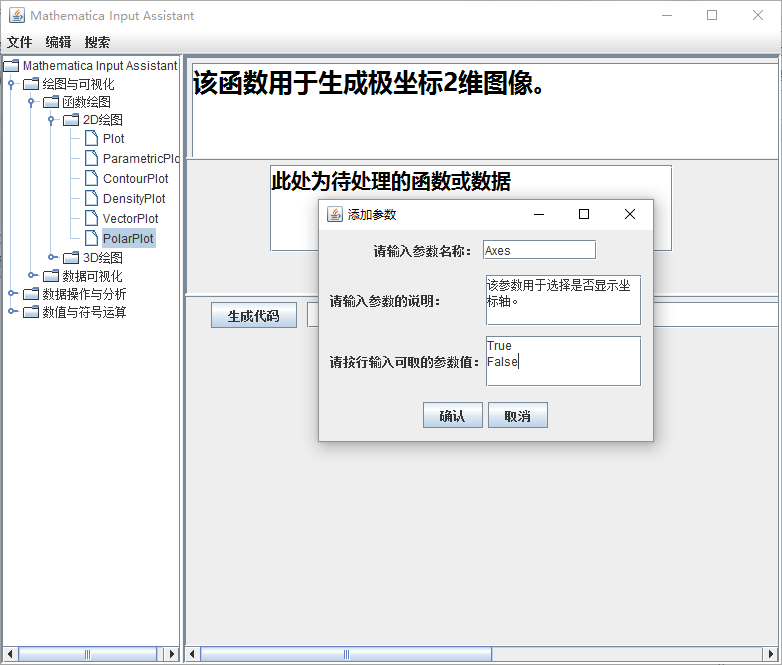
\includegraphics[width=3in]{13.png}
	                \caption{添加参数}
	                \label{pic:GUIPack}
	                \end{minipage}
            	\end{figure}

            	\begin{figure}[!h]
	                \begin{minipage}[b]{0.45\textwidth}
	                \centering
	                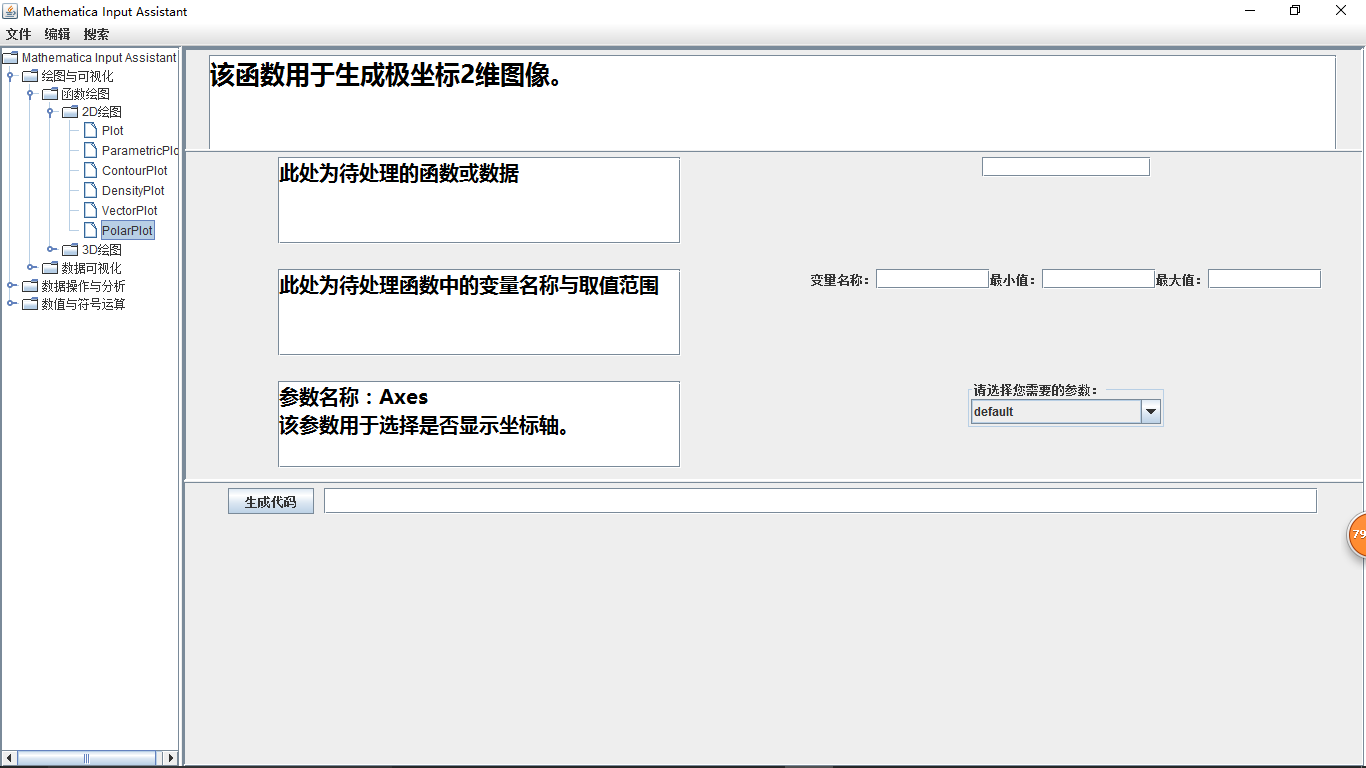
\includegraphics[width=3in]{14.png}
	                \caption{添加自变量取值范围}
	                \label{pic:MathPack}
	                \end{minipage}%
	                \hspace{0.1\textwidth}%
	                \begin{minipage}[b]{0.45\textwidth}
	                \centering
	                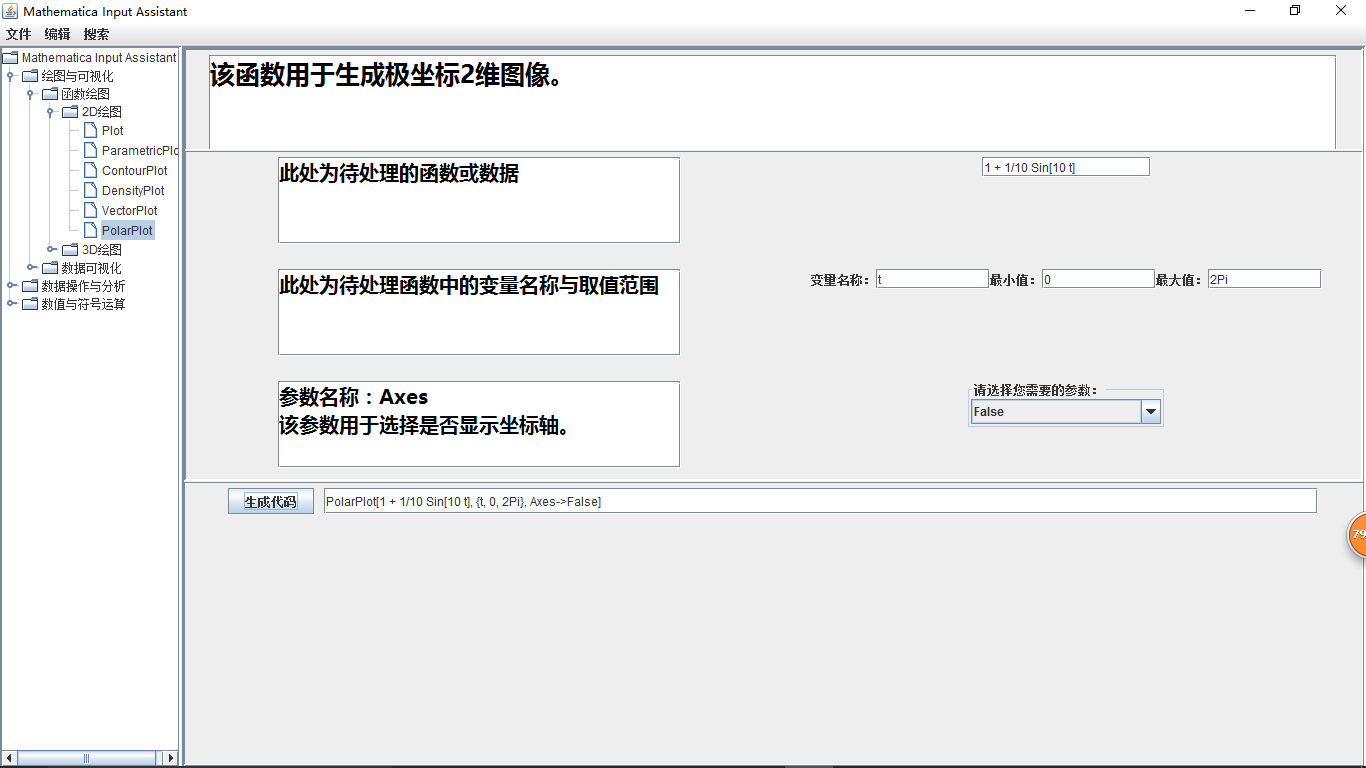
\includegraphics[width=3in]{15.png}
	                \caption{按图输入}
	                \label{pic:GUIPack}
	                \end{minipage}
            	\end{figure}

            	\begin{figure}[!h]
                	\centering
                	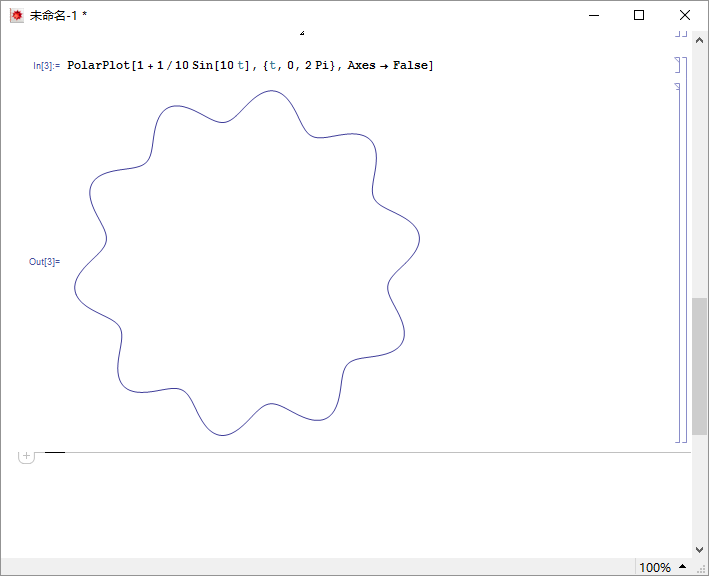
\includegraphics[width=4in]{16.png}
                	\caption{拷入Mathematica中运行}    
                	\label{pic:MathObject}
            	\end{figure}
            	\bigskip
           \bigskip
    \section{搜索功能}
    点击菜单栏搜索按钮,弹出搜索对话框。

    \begin{figure}[!h]
                	\centering
                	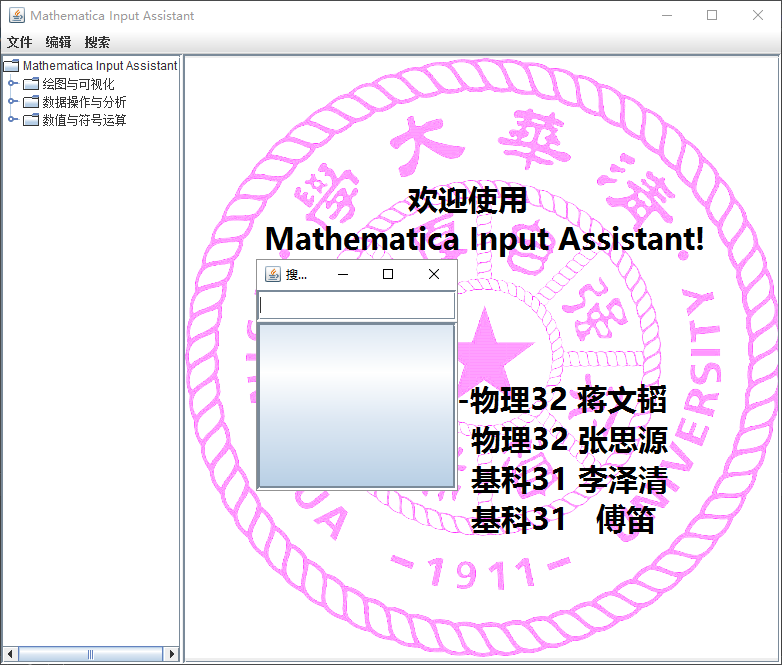
\includegraphics[width=4in]{17.png}
                	\caption{搜索框弹出测试}    
                	\label{pic:MathObject}
            	\end{figure}

            	输入p,搜索对话框如图显示;再输入l后,搜索对话框变化如图显示。

            					\begin{figure}[!h]
	                \begin{minipage}[b]{0.45\textwidth}
	                \centering
	                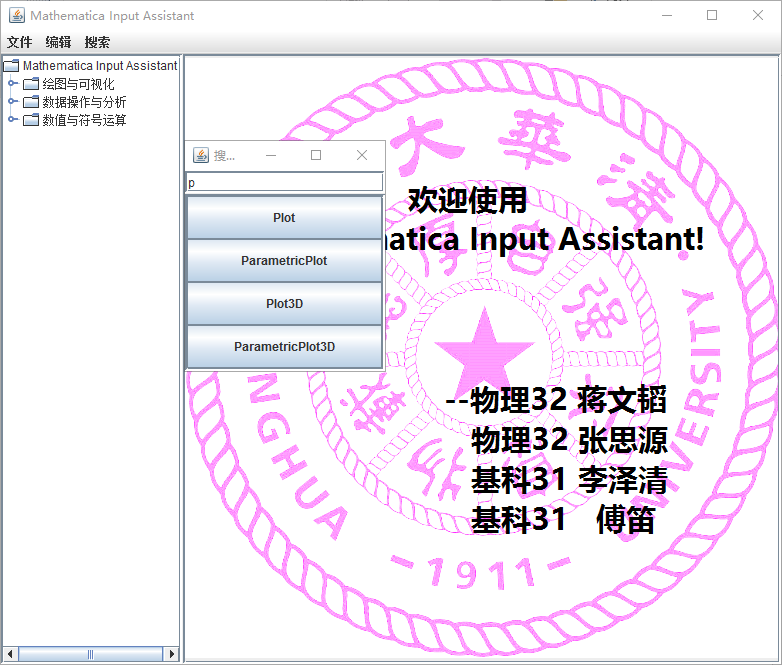
\includegraphics[width=3in]{18.png}
	                \caption{输入p}
	                \label{pic:MathPack}
	                \end{minipage}%
	                \hspace{0.1\textwidth}%
	                \begin{minipage}[b]{0.45\textwidth}
	                \centering
	                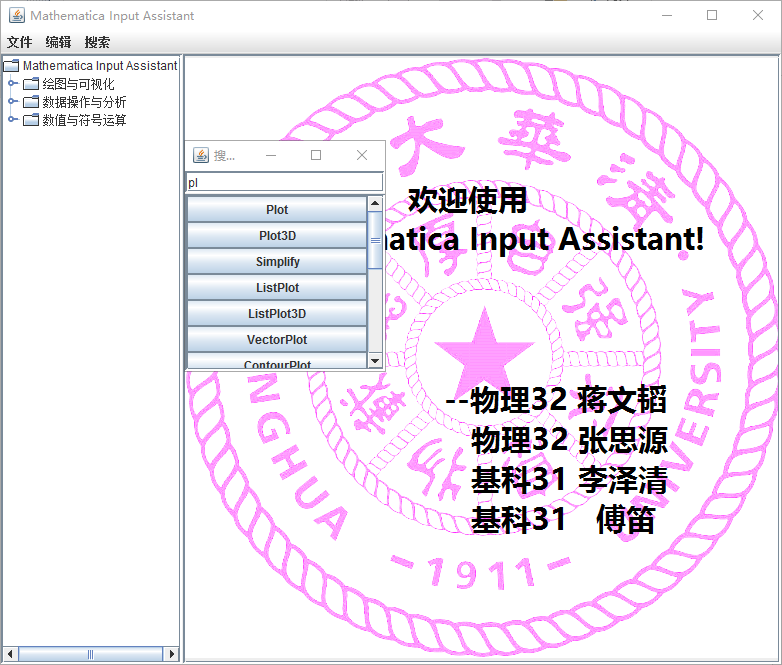
\includegraphics[width=3in]{19.png}
	                \caption{再输入l}
	                \label{pic:GUIPack}
	                \end{minipage}
            	\end{figure}



\end{document}